
% bayes-filter.tex

\documentclass[dvipdfmx,a4paper]{jsarticle}

\usepackage{docmute}

% settings.tex

\usepackage{atbegshi}
\AtBeginDvi{\special{pdf:tounicode 90ms-RKSJ-UCS2}}

\usepackage{amsmath}
\usepackage{amssymb}
\usepackage{amsfonts}
\usepackage{amsthm}
\usepackage{bm}
\usepackage{ascmac}
\usepackage{comment}
\usepackage{fancybox}
\usepackage{framed}
\usepackage{color}
\usepackage[dvipdfmx]{graphicx}
\usepackage{multicol}
\usepackage{multirow}
\usepackage{pdflscape}
\usepackage{verbatim}

\usepackage{url}
\urlstyle{same}

\DeclareMathOperator*{\argmax}{arg\,max}
\DeclareMathOperator*{\argmin}{arg\,min}
\DeclareMathOperator{\Tr}{Tr}
\DeclareMathOperator{\KL}{KL}
\DeclareMathOperator{\diag}{diag}
\DeclareMathOperator{\bel}{bel}
\DeclareMathOperator{\belp}{\overline{bel}}

\usepackage[T1]{fontenc}
\usepackage[utf8]{inputenc}

\usepackage{algorithm}
\usepackage{algpseudocode}
\usepackage{algorithmicx}

\renewcommand{\algorithmicrequire}{\textbf{Input:}}
\renewcommand{\algorithmicensure}{\textbf{Output:}}

\makeatletter
\renewcommand{\ALG@name}{アルゴリズム}
\makeatother

\algnewcommand{\Initialize}[1]{
	\State \textbf{Initialize:}
 	\State \hspace*{\algorithmicindent}\parbox[t]{0.8\linewidth}{\raggedright #1}}


\usepackage{geometry}
\geometry{left=19.05mm,right=19.05mm,top=19.05mm,bottom=19.05mm}

\title{ベイズフィルタ}
\author{にゃーん}
\date{\today}

\begin{document}

\maketitle

この資料は、文献~\cite{Thrun07}の2.3節と2.4節をまとめたものです。

\section{ロボットと環境の相互作用}
\subsection{ロボットの状態}
ロボットにおける\textbf{状態}として、ここではグローバル座標系(地図座標系)におけるロボットの\textbf{位置}と\textbf{向き}を考える。3次元の空間を動き回るロボットの場合、その状態は6変数あれば表現できる。6変数のうち3変数はロボットの位置で、直交座標系における$x$座標、$y$座標、$z$座標、そして残りの3変数はロボットの向きで、ロール角、ピッチ角、ヨー角となる。平面上を動き回るロボットの場合、その状態は3変数で表現できる。位置には直交座標系における$x$座標と$y$座標、向きには回転角(ヨー角)が用いられる。ロボットの状態は変数$x$で表す。

\subsection{ロボットの制御}
ロボットに制御が加わることによって、ロボットの状態$x$は変化する。ロボットの制御は、例えば並進速度$v$と回転速度$\omega$の2つで表現できる。ロボットに与える制御は変数$u$で表す。

\subsection{ロボットの観測}
ロボットは、自身に装備されたセンサを用いて、周囲の環境を計測する。計測データとしては、例えばレーザレンジファインダによって取得されたスキャンデータなどが挙げられる。ロボットの計測データは変数$z$で表す。

\subsection{確率によるモデル}
ロボットの状態$x$、制御$u$、計測$z$の関係は、図\ref{fig:dynamic-bayes-network}に示すような確率モデルとして表現できる。ここでは離散的な時刻$t = 0, 1, \cdots$において変数が記述されるとする。時刻$t$におけるロボットの状態、制御、計測をそれぞれ$x_t$、$u_t$、$z_t$とする。時刻$t - 1$において、ロボットは状態$x_{t - 1}$にある。時刻$t$で、ロボットに制御$u_t$が加わって、ロボットは状態$x_{t - 1}$から状態$x_t$へと遷移する。この状態遷移の後に、ロボットはセンサから計測データ$z_t$を得る。従って、ロボットに対する制御の後に、センサによる計測が起こる。図\ref{fig:dynamic-bayes-network}において、灰色に塗られた変数(制御と計測)は既知のものであり、ロボットはその値を入手できる。本当に知りたいのは白色の変数(状態)であるが、直接表には現れない(灰色の変数を介して間接的に現れる)ので、ベイズフィルタなどのアルゴリズムを駆使して、既知の変数から推定する必要がある。\newline

\begin{figure}[htbp]
	\centering
	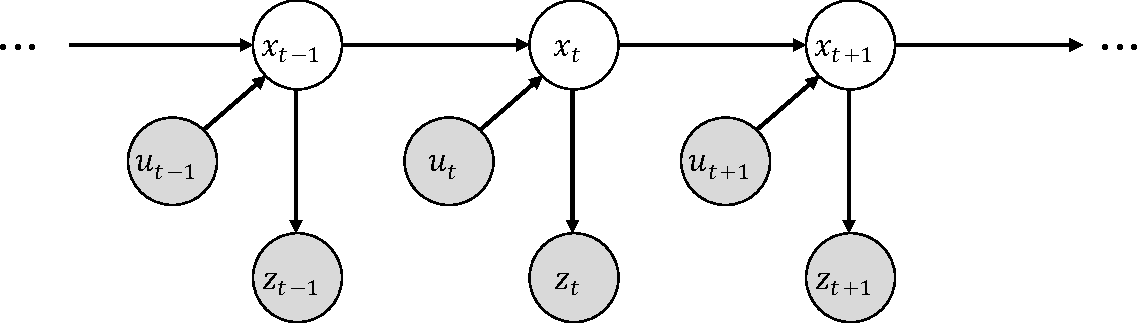
\includegraphics[keepaspectratio, scale=0.75]{figures/dynamic-bayes-network.pdf}
	\caption{ロボットの確率モデル}
	\label{fig:dynamic-bayes-network}
\end{figure}

時刻$t$におけるロボットの状態$x_t$は、過去の全ての状態や計測、制御に依存すると考えられるので、ロボットの状態$x_t$を表す確率分布は$p(x_t | x_{0 : t - 1}, z_{1 : t - 1}, u_{1 : t})$のように書ける。しかし、ここではマルコフ性を仮定し、ロボットの現在の状態$x_t$は、直前の状態$x_{t - 1}$と、ロボットに与えられた制御$u_t$のみによって決まると考える。一時刻前の状態$x_{t - 1}$には、それよりも前の状態$x_{0 : t - 2}$や、計測$z_{1 : t - 1}$、制御$u_{1 : t - 1}$に関する情報が全て詰まっている。それゆえ、変数$x_t$を決めるうえでは、直前の状態$x_{t - 1}$と現在の制御$u_t$さえあれば十分だということを示唆している。従って、$x_t$の確率分布については次の等式が仮定される。
\begin{equation}
	p(x_t | x_{0 : t - 1}, z_{1 : t - 1}, u_{1 : t}) = p(x_t | x_{t - 1}, u_t) \label{eq:transition-prob}
\end{equation}

時刻$t$におけるロボットの計測$z_t$についても、上記と同様にマルコフ性が仮定される。これより、$z_t$は過去の全ての状態や計測、制御には依存するのではなく、ロボットの現在の状態$x_t$にのみ影響を受ける。図\ref{fig:dynamic-bayes-network}からも明らかなように、現在の状態$x_t$には、それ以前の全ての状態$x_{0 : t - 1}$や、計測$z_{1 : t - 1}$、制御$u_{1 : t}$に関する情報が凝縮されているので、$z_t$を得るうえでは、$x_t$以外の変数は不要となる。従って、$z_t$の確率分布については次の等式が仮定される。
\begin{equation}
	p(z_t | x_{0 : t}, z_{1 : t - 1}, u_{t : t}) = p(z_t | x_t) \label{eq:observation-prob}
\end{equation}

$x_t$に関する確率分布$p(x_t | x_{t - 1}, u_t)$は\textbf{状態遷移確率}とよばれる。ロボットの状態が$x_{t - 1}$にあって、制御$u_t$が加わったときに、どの状態に遷移し得るのかを表す。状態$x_t$は決定論的な関数ではなく、確率分布によって記述されるので、制御や状態に加わるノイズの影響が、最初から考慮されている。$z_t$に関する確率分布$p(z_t | x_t)$は\textbf{計測確率}とよばれる。ロボットが状態$x_t$にいるときに、どのような計測データ$z_t$が得られるのかを表す。計測$z_t$も確率分布として記述されるので、ノイズの影響が考慮される。図\ref{fig:dynamic-bayes-network}は、確率変数間の依存関係を表しており、現在の状態$x_t$は直前の状態$x_{t - 1}$と制御$u_t$に、計測$z_t$は現在の状態$x_t$に依存している。状態$x_t$は次の状態$x_{t + 1}$にのみ影響を及ぼす。

\subsection{ロボットの信念}
前節から、ロボットの状態変数と、制御や計測との関係が、2つの確率分布$p(x_t | x_{t - 1}, u_t)$、$p(z_t | x_t)$として表現された。しかし本当にやりたいのは、実際の数値として入手可能な制御や計測から、陽には現れないロボットの状態を推定することである。ロボットの現在の状態$x_t$を推定するために、以下のような確率分布$\bel(x_t)$を考える。
\begin{equation}
	\bel(x_t) = p(x_t | z_{1 : t}, u_{1 : t})
\end{equation}
$\bel(x_t)$は、過去全ての計測$z_{1 : t}$と制御$u_{1 : t}$が明らかになっているときの、状態$x_t$に関する確率分布である。従って$\bel(x_t)$は、時刻$t$における計測$z_t$が\textbf{得られた後}に求められる。このことから、$\bel(x_t)$は\textbf{事後信念}とよばれる。計測$z_t$が反映される前の\textbf{事前信念}として、次の$\belp(x_t)$を考えることができる。
\begin{equation}
	\belp(x_t) = p(x_t | z_{1 : t - 1}, u_{1 : t})
\end{equation}
ロボットが計測$z_t$を得る前に、ロボットは事前信念$\belp(x_t)$に基づいて現在の状態$x_t$を推定する。次に計測$z_t$が観測されると、$z_t$を使って、現在の状態$x_t$に関する予測を$\belp(x_t)$から$\bel(x_t)$へと更新できる。$z_t$を用いて、$\belp(x_t)$から$\bel(x_t)$を計算し、現在の状態$x_t$に関する確率分布を更新することを、\textbf{修正}や\textbf{計測更新}という。次の制御$u_{t + 1}$が与えられると、現在の$\bel(x_t)$と$u_{t + 1}$から、事前信念$\belp(x_{t + 1})$が新たに計算される。そして、次の観測$z_{t + 1}$によって、事前信念$\belp(x_{t + 1})$から事後信念$\bel(x_{t + 1})$が計算されて、状態$x_{t + 1}$に関する推定は修正される。制御と計測によって、このような信念分布$\belp(x_t), \bel(x_t)$の計算が綿々と続くことになる。

\section{ベイズフィルタ}
\subsection{アルゴリズム}
制御と計測から信念分布$\bel(x_t)$を計算するための一般的な枠組みとして、ベイズフィルタがある。カルマンフィルタやパーティクルフィルタは、全てベイズフィルタの派生形として捉えられる。ベイズフィルタは以下のアルゴリズム\ref{alg:bayes-filter}のように記述される。時刻$t - 1$における事後信念$\bel(x_{t - 1})$から、時刻$t$における事後信念$\bel(x_t)$を計算するためのものである。

\begin{algorithm}[H]
	\caption{ベイズフィルタ}
	\label{alg:bayes-filter}
	\begin{algorithmic}[1]
		\Require
			\Statex 時刻$t - 1$における事後信念$\bel(x_{t - 1})$
			\Statex 時刻$t$における制御$u_t$
			\Statex 時刻$t$における計測$z_t$
		\Ensure
			\Statex 時刻$t$における事後信念$\bel(x_t)$ \newline
		
		\For{all $x_t$}
			\State $\belp(x_t) = \displaystyle \int p(x_t | x_{t - 1}, u_t) \bel(x_{t - 1}) dx_{t - 1}$ \label{alg:bayes-filter-prior-belief}
			\State $\bel(x_t) = \eta \ p(z_t | x_t) \belp(x_t)$ \label{alg:bayes-filter-posterior-belief}
		\EndFor
	\end{algorithmic}
\end{algorithm}

ベイズフィルタは2つの大まかなステップ、\textbf{予測}と\textbf{修正}に分けられる。アルゴリズムの\ref{alg:bayes-filter-prior-belief}行目は予測ステップを表している。制御$u_t$を用いて、直前の事後信念$\bel(x_{t - 1})$から、現在の状態$x_t$に関する事前信念$\belp(x_t)$が計算され、$x_t$に対する予測が行われる。計算は、2つの確率分布、状態遷移確率$p(x_t | x_{t - 1}, u_t)$と直前の事後信念$\belp(x_{t - 1})$の積の、変数$x_{t - 1}$に関する積分である。
\begin{equation}
	\belp(x_t) = \int p(x_t | x_{t - 1}, u_t) \bel(x_{t - 1}) dx_{t - 1}
\end{equation}
状態が離散的であれば、積分は次のように総和に置き換えられる。即ち、時刻$t - 1$で取り得る全ての状態$x_{t - 1}$について、2つの確率分布の積$p(x_t | x_{t - 1}, u_t) \bel(x_{t - 1})$を足し合わせたものになる。
\begin{equation}
	\belp(x_t) = \sum_{x_{t - 1}} p(x_t | x_{t - 1}, u_t) \bel(x_{t - 1})
\end{equation}
アルゴリズムの\ref{alg:bayes-filter-posterior-belief}行目は修正ステップを表している。計測$z_t$を用いて、現在の事前信念$\belp(x_t)$から事後信念$\bel(x_t)$が計算される。即ち、予測ステップで得られていた$x_t$に対する事前信念$\belp(x_t)$が、$z_t$の観測によって、より精度の高い事後信念$\bel(x_t)$へと更新される。計算は、2つの確率分布、計測確率$p(z_t | x_t)$と事前信念$\belp(x_t)$の積である。$\bel(x_t)$が確率としての条件を満たす(積分の結果が$1$になる)ように、正規化定数$\eta$を乗算する。
\begin{equation}
	\bel(x_t) = \eta \ p(z_t | x_t) \belp(x_t)
\end{equation}
ベイズフィルタを使って計算を始めるためには、初期状態$x_0$における信念$\bel(x_0)$が必要である。初期状態が明らかであれば、$x_0$に全ての確率密度が集中したデルタ関数や、$x_0$の周囲のごく狭い範囲に確率密度が集中した、分散が非常に小さい正規分布を$\bel(x_0)$として利用できる。初期状態が不明であれば、$x_0$の全定義域にわたって、確率密度が定数となる一様分布を$\bel(x_0)$として採用できる。\newline

ベイズフィルタでは、取り得る全ての状態$x_t$について、上式のような総和と積分を計算しなければならない。予測ステップにおいて、$x_{t - 1}$の全定義域にわたる積分を厳密に(解析的に)実行できるか、あるいは有限回の和に置き換えて計算できる必要がある。取り得る状態$x_t$が連続的であれば、全ての$x_t$において$\belp(x_t)$と$\bel(x_t)$を計算するのは不可能である。状態$x_t$が離散的であっても、状態空間が広い(取り得る状態$x_{t - 1}$の数が大きい)場合は、計算量の観点から、予測ステップでの総和の計算が困難になる。従って、状態空間が非常に狭いという、ごく限られた場合にしか、上記に示すベイズフィルタを適用できないと考えられる。

\subsection{アルゴリズムの導出}
ここでは、時刻$t - 1$における事後信念$\bel(x_{t - 1}) = p(x_{t - 1} | z_{1 : t - 1}, u_{1 : t - 1})$から、時刻$t$における事後信念$\bel(x_t) = p(x_t | z_{1 : t}, u_{1 : t})$が計算できることを示す。但し、初期状態$x_0$に関する事後信念$\bel(x_0)$は既知とする。時刻$t - 1$において、事後信念$\bel(x_{t - 1})$がベイズフィルタにより正しく計算できると仮定する。時刻$t$における事後信念$\bel(x_t)$は、ベイズの定理から
\begin{eqnarray}
	\bel(x_t) &=& p(x_t | z_{1 : t}, u_{1 : t}) \nonumber \\
	&=& \frac{p(z_t | x_t, z_{1 : t - 1}, u_{1 : t}) p(x_t | z_{1 : t - 1}, u_{1 : t})}{p(z_t | z_{1 : t - 1}, u_{1 : t})} \qquad (\because ベイズの定理) \\
	&=& \eta \ p(z_t | x_t, z_{1 : t - 1}, u_{1 : t}) p(x_t | z_{1 : t - 1}, u_{1 : t})
\end{eqnarray}
と変形できる。ここで$\eta = p(z_t | z_{1 : t - 1}, u_{1 : t})$は、状態$x_t$には依存しないため、定数として扱っている。式\ref{eq:observation-prob}でみたように、現在の観測$z_t$は、状態$x_t$のみによって決まり、それ以外の変数とは独立なので
\begin{equation}
	\bel(x_t) = \eta \ p(z_t | x_t) p(x_t | z_{1 : t - 1}, u_{1 : t})
\end{equation}
とできる。右側の項$p(x_t | z_{1 : t - 1}, u_{1 : t})$は事前信念$\belp(x_t)$であるので、結局次のようになる。
\begin{equation}
	\bel(x_t) = \eta \ p(z_t | x_t) \belp(x_t)
\end{equation}
これはアルゴリズムの\ref{alg:bayes-filter-posterior-belief}行目に示した、修正ステップを表している。\newline

時刻$t$における事前信念$\belp(x_t)$は、以下のように$x_{t - 1}$についての周辺化として
\begin{eqnarray}
	\belp(x_t) &=& p(x_t | z_{1 : t - 1}, u_{1 : t}) \nonumber \\
	&=& \int p(x_t | x_{t - 1}, z_{1 : t - 1}, u_{1 : t}) p(x_{t - 1} | z_{1 : t - 1}, u_{1 : t}) dx_{t - 1} \qquad (\because 周辺化)
\end{eqnarray}
と記述できる。式\ref{eq:transition-prob}でみたように、現在の状態$x_t$は、直前の状態$x_{t - 1}$及び制御$u_t$のみから決定されるので
\begin{equation}
	\belp(x_t) = \int p(x_t | x_{t - 1}, u_t) p(x_{t - 1} | z_{1 : t - 1}, u_{1 : t}) dx_{t - 1}
\end{equation}
とできる。右辺の項$p(x_{t - 1} | z_{1 : t - 1}, u_{1 : t})$について、$x_{t - 1}$は時刻$t - 1$以前の変数から決まるため、未来に得られる制御$u_t$は条件変数から取り去ることができる。即ち$p(x_{t - 1} | z_{1 : t - 1}, u_{1 : t}) = p(x_{t - 1} | z_{1 : t - 1}, u_{1 : t - 1})$となるから
\begin{eqnarray}
	\belp(x_t) &=& \int p(x_t | x_{t - 1}, u_t) p(x_{t - 1} | z_{1 : t - 1}, u_{1 : t - 1}) dx_{t - 1} \\
	&=& \int p(x_t | x_{t - 1}, u_t) \bel(x_{t - 1}) dx_{t - 1}
\end{eqnarray}
とできる。これはアルゴリズムの\ref{alg:bayes-filter-prior-belief}行目に示した、予測ステップを表している。\newline

ベイズフィルタを示す際に、マルコフ性の仮定が重要な役割を果たしている。ベイズフィルタを実行するためには、状態遷移確率$p(x_t | x_{t - 1}, u_t)$、計測確率$p(z_t | x_t)$、そして初期信念$\bel(x_0)$が必要である。制御$u_t$と計測$z_t$、直前の事後信念$\bel(x_{t - 1})$を入力として取り、過去の全ての制御$u_{1 : t}$と計測$z_{1 : t}$で条件付けられた、現在の状態$x_t$に関する事後信念$\bel(x_t)$を出力として返す。計測確率$p(z_t | x_t)$と状態遷移確率$p(x_t | x_{t - 1}, u_t)$は、ロボットや環境の特性に応じて適切にモデル化される。

\bibliographystyle{plain}
\bibliography{bayes-filter}

\end{document}
